% V12 projection; v11 source observations and generated table remain immutable.
\subsection{New public-software executions}
Thirty fresh process runs on six upstream projects record 151,380 check
executions. Table~\ref{tab:v11-cohort} reports one held-out run per project;
the second has the same counts. These counts are execution observations,
not independent projects. Only five projects (25 runs, 16,640 check
executions) are admitted to the compiler comparison. All five have identical
completion orders and ordered wave partitions across runs 0--4. Thus the
held-out costs measure repetition of observed completion patterns, not
prediction of new patterns. attrs' 33 failures concern this environment
(including mypy compatibility) and are retained without calling them
upstream bugs. Skips, xfails and xpasses remain unknown.

\begin{table}[t]\centering\footnotesize
\caption{New complete suites. Counts per held-out run; five runs per project.
P/F/U are PASS/FAIL/UNKNOWN.}\label{tab:v11-cohort}
\begin{tabular}{@{}lrrrr@{}}\toprule
Project & Checks & P & F & U\\\midrule
Click & 761 & 739 & 0 & 22 \\
Jinja & 909 & 909 & 0 & 0 \\
Packaging & 26,948 & 26,948 & 0 & 0 \\
Pluggy & 124 & 124 & 0 & 0 \\
attrs & 1,432 & 1,391 & 33 & 8 \\
ExceptionGroup & 102 & 91 & 0 & 11 \\
\bottomrule\end{tabular}
\end{table}

Raw collection order varied in Packaging. Before any layout-cost analysis,
a dated correction created separate canonical-registry copies, retaining
the raw records and every scheduled/completed ID unchanged. Jinja's missing
Trio test dependency was repaired before its five retained runs; the original
failed attempt is preserved. Source files remain hash-verified. The original
environment identifier binds Python/platform, not all dependencies.
A post-hoc inventory records the repair and duplicate package metadata;
it cannot retroactively establish a complete contemporaneous environment
identity. Each representation comparison still uses the same persisted
input trace.

\subsection{Held-out topology costs}
Table~\ref{tab:v11-gains} compares frozen refined selections to historical
compact selection. The primary cap32 method improves two of five admitted
project cases and ties three. The cap64 results were designated secondary
before collection; they do not replace the primary endpoint. Both methods
are fitted on runs 0--1, selected on run 2 and scored on runs 3--4.
All selected layouts were hash-frozen before those held-out costs were opened.
\begin{table}[t]\centering\footnotesize
\caption{Held-out padded-byte reduction (\%) relative to the historical
compact catalogue. Construction is included. UNKNOWN is not a tie.}
\label{tab:v11-gains}
\begin{tabular}{@{}lrr@{}}\toprule
Project & Cap32 primary & Cap64 secondary\\\midrule
Click & 1.493 & 17.219 \\
Jinja & 0.177 & 15.996 \\
Packaging & \multicolumn{2}{c}{UNKNOWN} \\
Pluggy & 0.000 & 18.695 \\
attrs & 0.000 & 0.000 \\
ExceptionGroup & 0.000 & 18.690 \\
\bottomrule\end{tabular}
\end{table}

The positive secondary reductions range from 16.00\% to 18.69\%; attrs
retains its incumbent. The gain is a measured topology-refinement effect
at the stated order, not a causal demonstration that higher-order information
alone explains it. Figure~\ref{fig:v11-boundaries} separates this representation
endpoint from service time.

Packaging has 26,948 declared checks. One dense float64 affinity matrix
alone would require about 5.81\,GB (5.41\,GiB); dictionary/heap clustering
needs more. The compiler therefore records optimization UNKNOWN under its
2\,GiB campaign budget, retains every ID and supplies an explicitly labeled
compact fallback only for conformance/scaling records. It is excluded from
the five-project compiler comparison rather than being counted as a tie.

\subsection{Transfer to historical-source regressions}
An additional frozen plan selects eleven real upstream fix commits by
syntax and history, transplants their parent production modules into
isolated release snapshots, and runs unchanged release tests with
stop-on-first-failure. Nine cases execute; eight preserve the release
registry. Two startup incompatibilities and one changed semantic ID set
are VOID for paired analysis. One matching Packaging case remains UNKNOWN
because fitting was not admitted. The seven measured transfers yield
two primary wins, three ties and two losses. In particular, Click's
primary layout costs 2.09\% and 2.58\% more than the historical compact layout
on its two partial trajectories. The retained all-pass Jinja case is
unrevealing, rather than excluded.

These are exploratory source transplants under a newer fixed test contract,
not executions of each native historical parent suite or a certified
natural-bug benchmark. They share project tests and supply no extra
independent project replication. No source-transfer outcome changes the
frozen layout. The losses demonstrate that training monotonicity and a
successful repeated-snapshot holdout do not ensure benefit after a source
or stopping-pattern change.

\subsection{Whole-trajectory service accounting}
The original comparison admits ten traces from five projects at the fixed 2,048-check
service budget; both complete Packaging inputs remain UNKNOWN without
subsampling. It executes four arms, three randomized-order repeats and
cold/warm queries at initial, intermediate and final snapshots.
All 5,040 service/oracle answer checks agree,
including exact epoch and missing-check disclosure. Each arm delivers the
same complete answer bytes under the common deterministic codec.

\begin{table}[t]\centering\footnotesize
\caption{Local service operation time (ms), mean of two per-case medians over
three whole-trajectory timing repeats. Builds, all ingests, queries and
codec work are included. Layout fitting is reported separately.
No network or agent inference occurs.}\label{tab:v11-time}
\begin{tabular}{@{}lrrr@{}}\toprule
Project & Indexed & Counters & HACT32\\\midrule
Click & 392.1 & 422.4 & 996.3 \\
Jinja & 555.0 & 527.4 & 1236.8 \\
Pluggy & 38.5 & 37.6 & 56.4 \\
attrs & 1067.1 & 1169.5 & 2833.9 \\
ExceptionGroup & 30.2 & 29.1 & 41.8 \\
\bottomrule\end{tabular}
\end{table}

These original timings include observational serialization for byte
counters, including whole-state serialization at every ingest. They measure
the instrumented prototype rather than isolated functional service costs.
All 30 matched timing-repeat HACT32/counter ratios exceed one
(range 1.216--2.850); repeated timings are descriptive, not independent
project replications. The separately frozen observer ablation below
measures the effect of this instrumentation.

The selected HACT service is slower than the maintained-counter ledger in
every admitted project case. Its ratio of mean case-median operation times
ranges from 1.44 to 2.42 on this host. Additional layout fitting and manifest
admission cannot turn those observed service losses into a positive
end-to-end speedup. The table times precompiled service execution and does
not hide fitting inside common checker time. Compiler receipts retain
separate one-time fit/selection measurements; their concurrent collection
load makes them descriptive rather than controlled speedup estimates.
The outcome supports a maintained ledger as the initial service baseline
for these requests, while preserving the distinct within-format packet
savings above.

\begin{figure*}[t]\centering
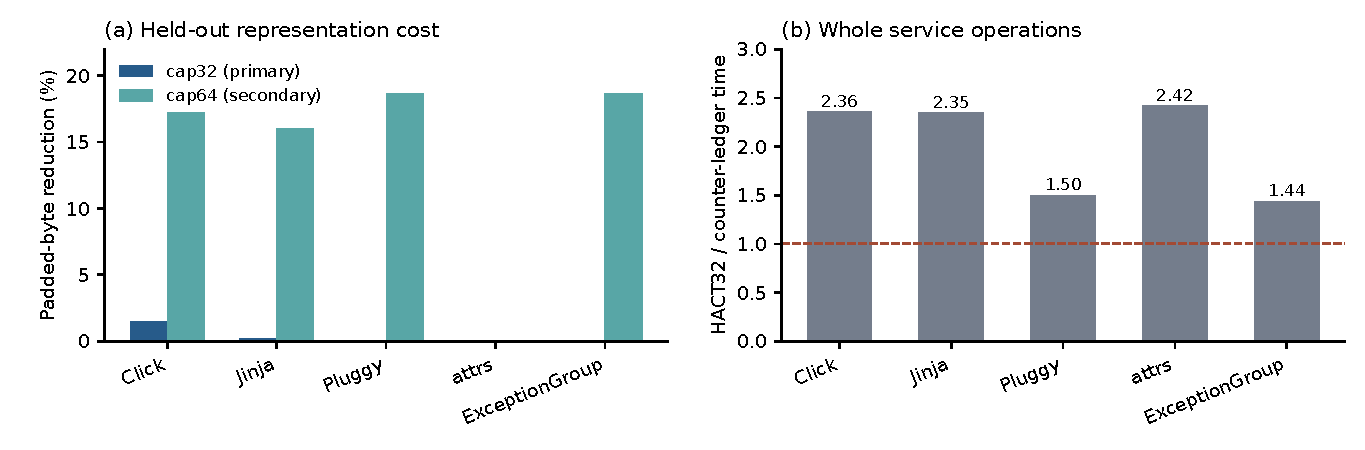
\includegraphics[width=.96\textwidth]{figures/v11_boundaries.pdf}
\caption{Different endpoints lead to different adoption decisions.
Left: primary and prespecified secondary held-out padded-byte savings.
Right: original instrumented precompiled service time of primary HACT divided by the
maintained-counter ledger; values above one are slower. Packaging is
UNKNOWN under resource admission and is not plotted as zero.}
\label{fig:v11-boundaries}
\end{figure*}

\subsection{Controlled dispatch-shift transfer}
The new campaign contains 36 complete suite executions and 20,580 check
executions. Six initial ExceptionGroup runs are VOID for cost analysis:
the profiler observed an ignored build-generated version module absent from
the frozen tracked-source inventory. Their raw records are retained. A
separate child protocol freezes that module before rerunning all six
predeclared schedules, without changing tests, seeds, layouts or endpoints.
The resulting admitted comparison has 30 executions and 19,968 checks over
five projects; it does not silently reclassify the original exclusions.
All admitted runs retain the original registry and status counts, including
attrs' environment-related failures.

\begin{table}[t]\centering\footnotesize
\caption{Primary cap32 padded-byte reduction (\%) under controlled dispatch
shifts relative to historical compact selection. Ranges span the three
fixed seeds; negative values are losses. No refitting.}
\label{tab:v12-shifts}
\begin{tabular}{@{}lrr@{}}\toprule
Project & File groups & Individual items\\\midrule
Click & -4.85 to -3.33 & -9.01 to -8.94 \\
Jinja & 0.15 to 0.17 & -0.12 to -0.07 \\
Pluggy & 0.00 & 0.00 \\
attrs & 0.00 & 0.00 \\
ExceptionGroup & 0.00 & 0.00 \\
\bottomrule\end{tabular}\end{table}

Against the historical selected comparator, file-group shuffling gives
three primary wins, nine ties and three losses; item shuffling gives zero
wins, nine ties and six losses. The comparison unit here is a scheduled
process, not an independent project. The small Jinja file-group gain survives,
whereas Click loses under both shifts. The three ties are projects whose
primary selection did not change. This directly limits the inference from
the repeated-pattern holdout. Every seed, all four frozen layouts, the
original compact comparison and secondary cap64 prices are retained in
the artifact. Neither the intervention nor the analytical witness identifies
natural deployment prevalence or a causal higher-order benefit.

\subsection{Service costs with byte observers disabled}
The separate ablation completes 240 arm executions: ten held-out traces,
three repeats and eight arms. All 10,080 raw-oracle/common-codec answer
checks agree; the two complete Packaging traces remain UNKNOWN under the
unchanged service budget. Table~\ref{tab:v12-observer} compares the same
primary layout to the maintained-counter ledger within each new timing block.

\begin{table}[t]\centering\footnotesize
\caption{Observer ablation. Disabled columns are mean case-median operation
times (ms); ratios compare HACT32 with counters in the same campaign.
Inst.=original instrumentation; off=byte observers disabled.}
\label{tab:v12-observer}
\begin{tabular}{@{}lrrrr@{}}\toprule
& \multicolumn{2}{c}{Observers off (ms)} & \multicolumn{2}{c}{HACT/counter}\\
Project & Counter & HACT32 & Inst. & Off\\\midrule
Click & 137.9 & 429.2 & 2.16 & 3.11 \\
Jinja & 140.3 & 446.1 & 2.23 & 3.18 \\
Pluggy & 23.0 & 37.1 & 1.45 & 1.61 \\
attrs & 261.3 & 924.9 & 2.64 & 3.54 \\
ExceptionGroup & 20.3 & 39.0 & 1.43 & 1.92 \\
\bottomrule\end{tabular}\end{table}

Removing observational serialization reduces absolute service time but
does not reverse the comparison. Primary HACT is slower than counters
in every paired timing block under both instrumentation states. With
observers disabled, the project ratios of mean case medians range from
1.61 to 3.54; individual paired-block ratios range from
1.135 to 4.630. These are descriptive host-specific
ranges, not confidence intervals. The disabled variant retains functional
packet serialization, evidence digests, record copies, validation, caches
and codec round trips. It is a controlled prototype ablation, not an optimized
production implementation. The negative service result therefore survives
the identified observer-cost confound for this demand.

